
\chapter{基于改进的Q-learning算法在不定期直复营销中的研究}

普通的监督学习方法和非监督学习方法在处理序列化决策的问题时,只能最大化单个独立事件的即时收益,无法顾及序列上不同决策点之间的相互影响,因而不能很好地处理直复营销这种序贯决策问题。而强化学习算法在学习时,因为考虑到了序列中的延迟影响并且以长期收益最大化作为优化目标,十分擅长处理序贯决策问题,所以本章选择使用强化学习的方法对该问题进行研究。首先,使用经典的强化学习算法Q-learning对直复营销场景进行建模,然后针对营销时间间隔不固定会给奖赏信号带来噪声影响这一问题,提出Interval-Q算法。并且,为了提高在大规模数据集下模型的训练效率,在Q采样方法的基础上,引入TD偏差,提出了基于TD偏差的Q采样方法。最后,在不定期直邮营销的仿真环境中进行模型的评估,以此来验证所提方法的有效性。

\section{研究动机}
\subsection{直复营销与序贯决策}
如本文第一章所述,在直复营销场景中的每个营销时刻点,营销人员都需要根据客户的个人信息和其之前的交互历史,做出应该对哪些客户进行营销的决策。而监督学习和非监督学习方法在求解该问题时,都仅仅只能考虑到最大化单个独立事件的即时收益,并不能保证在一段时间上的长期收益最大化,这与直复营销所追求的最终目标不符。
% 解决这个问题常用的算法有传统的分类算法和基于代价敏感的学习算法,然而这些算法在决策时

直复营销是一个序贯决策过程,即随着时间的推移,营销人员需要不断地做出营销决策,通常以长期收益最大化作为营销效果的评价指标。因此,在制定营销决策的时候,营销人员不仅需要考虑到每个决策行为的成本和其(即时)收益之间的关系,而且还要考虑到不同决策行为之间的相互影响。

考虑如下情景:在某次制定营销决策的时候,营销人员发现,如果此时对某位客户进行营销的话,其产生的估计收益会大于营销成本(即利润为负),那么营销人员就不会对这位客户进行营销了。然而,营销人员应该意识到,即使该客户在此次的营销活动中不会产生即时利润,但正是因为这一次的营销,可能会增加该客户在后续的营销活动中所产生的利润,甚至该利润值会很大,这样看来,此次对该顾客进行营销就很有必要了。所以,当营销人员进行营销决策时,有时候需要牺牲即时收益以获得长期收益最大化。反之亦然,如果频繁地对某一位高质量用户发送营销信息,则会降低该客户所能产生的期望收益,因为每一位客户在一段时间内消费能力是有限的。

\subsection{强化学习}
因为强化学习在学习过程中考虑到了序列中奖赏信号的延迟影响,并且以累积奖赏最大化作为学习目标。所以通过这种学习方式可以很好地处理直复营销决策中不同营销点之间的相互影响,进而达到长期收益最大化的目标,因此文献\citep{pednault2002sequential,archak2010budget,boutilier2016budget}等提出使用强化学习的思想来解决直复营销中的决策问题。但是,在上述相关工作中,以下问题仍然没有得到有效解决:在不定期直复营销场景中,各个营销点之间的时间间隔是不固定的,所以如果采用强化学习中传统累积奖赏的计算方式,就会给奖赏信号带来一定的噪声,从而影响了值函数的学习。另外,在实际应用中,随着数据规模的不断攀升,值函数的学习速度也会变慢,从而给强化学习在现实应用中带来很大的障碍。

本章针对以上两个问题进行分析,提出了相应的改进方法,以更好地解决直复营销问题。首先,利用马尔科夫决策过程,将直复营销问题建模为一个强化学习问题,并给出Q-learning算法解决该问题的框架;然后,为了解决营销决策点间的时间间隔不固定给奖赏信号带来的噪声影响,提出了Interval-Q算法;最后,为了适应在大批量数据下的学习任务,本文在Q采样的基础上,引入TD偏差,提出一种改进的Q采样方法,以提高值函数的学习效率。

\section{改进的Q-learning算法在直复营销中的建模}
在本节中,首先使用Q-learning算法对直复营销场景进行建模,构建一个可以解决直复营销问题的模型框架。然后,结合不定期直复营销中营销时间间隔不固定的问题,对Q-learning算法中值函数更新方法进行改进。接着,为了解决大规模数据集下模型更新的效率问题,在Q采样方法的基础上,提出了基于TD偏差的Q采样法。

\subsection{直复营销问题的形式化描述}
在本文的第二章中提到,强化学习问题可以使用如下马尔可夫决策过程来进行描述:在任意给定的时间点上,假设环境处于某个状态,当Agent采取一个行为时,它会收到一个有限的奖赏,并且环境会相应的转移到下一个状态。在这一过程中,Agent是以最大化累积奖赏作为行为选择的依据,且该奖赏通常是以累积折扣的形式表示。

同样地,在使用强化学习解决直复营销问题之前,首先要使用马尔科夫决策过程对直复营销问题进行形式化的描述:在某一时刻$t$,客户的状态为$S_{t}$,如果营销人员对其采取了营销行为$A_{t}$,那么该客户的状态会根据一定的转移概率转移到下一状态$S_{t+1}$,并且会产生一定的奖赏信息$R_{t}$。以上这个过程始终贯穿于客户和营销人员的营销交互之中,那么,可以使用$\{<S_{t},A_{t},R_{t}>\}_{t=1}^{\infty}$三元组来表示每一次的营销事件。
其中,客户的状态$S_{t}$可以使用客户在该时刻所具有的特征信息来表示,比如文献\citep{tkachenko2015autonomous}中提到的Recency-Frequency-Monetary(最近交易时间、交易频率和交易金额)等,不同的营销行为$A_{t}$代表企业不同类型的营销方式,客户在反馈中所产生的奖赏信息$R_{t}$是指该客户产生的净利润,也就是说,强化学习在解决直复营销的过程中是通过最大化每个客户的生命周期价值,进而来达到最大化企业长期收益的目的。

在强化学习模型的选择上,Q-learning算法(见算法$\ref{algo:algorithm_2}$)以其原理简单、实现方便的优点,在实际中得到广泛应用。所以,接下来本章将参考文献\citep{,pednault2002sequential}中的基于函数逼近的批强化学习方法,给出Q-learning算法解决直复营销问题的模型框架。

\subsection{基于Q-learning的直复营销模型构建}
在传统的Q-learning算法中,值函数其实是一个表格,其索引是状态或者状态行为对,值迭代更新实际上就是这张表格的迭代更新。所以,在Q-learning算法中存在一个假设是,问题的状态空间和行为空间不能太大。然而,在像直复营销这类复杂的现实问题中,为了合理准确地表示客户的状态信息,需要非常多的特征,其状态空间自然非常大,所以,如果这时依旧使用表格的形式进行值函数的表示并不现实。

如第二章所述,对于状态空间较大的问题可以通过函数逼近的方法进行值函数的估计。在强化学习的各类函数逼近方法中,基于非参数化函数逼近的方法虽然具有很好的表征能力,但是随着数据量的增多其计算量呈指数升高,所以,不适合直复营销这类含有大量训练数据的场景。而在参数化函数逼近方法中,基于非线性的逼近方法在逼近过程中存在着收敛困难的问题。因此,本章考虑使用参数化线性逼近的方法进行值函数的逼近。另外,在参数化线性逼近方法中,基于增量式学习方法在参数的更新过程随机性较大,尽管计算简单,但样本的利用效率不高,而基于批的更新方法尽管计算复杂,但是计算效率较高。所以,本节选择使用基于批更新的线性函数逼近方法。

\paragraph{分块线性函数逼近}
尽管线性逼近方法可以收敛到全局最优解,但是它的表征能力较弱,为了缓解这个问题,本节考虑使用分块逼近的思想以提高值函数的逼近精度:

Q值函数分块逼近模型:考虑具有连续状态空间$\mathcal{S}=\{S_{j}|j \in \mathbb{R}\}$和离散行为空间$\mathcal{A}=\{A_{i}\}_{i=1}^{K}$的强化学习问题,利用逼近模型$\mathcal{M}$对该问题的Q值函数进行建模。$\mathcal{M}=\{M_{i},\cdots,M_{K}\}$,其中$K$为离散行为个数。每个离散行为对一个子模型,子模型之间相互独立,称$\mathcal{M}$为Q值函数分块逼近模型。子模型可以采用任意的结构模型,若$K$个子模型结构相同,则称$\mathcal{M}$为同构分块逼近模型,否则称为异构分块逼近模型。

\begin{algorithm}[htbp]
\small
\SetAlgoLined
\SetKwRepeat{Repeat}{repeat}{until} 
\KwData{折扣因子$\gamma$,最大迭代轮数$P$,多项式次数$M$,原始总样本$D=\{e_{i}|i=1,\cdots,I\}$,其中$e_{i}=\{<S_{i,j}, A_{i,j}, R_{i,j}>|j=1,\cdots,l_{i}\}$,($D$表示样本集合,$e_{i}$表示第$i$个情节,$l_{i}$表示$e_{i}$的长度)}
\KwResult{输出最终的逼近模型:$Q^{(P)}$}

\For{all $e_{i} \in D$}{
	初始化第$i$个情节的数据:$D_{i}^{(0)}=\{<S_{i,j}, A_{i,j}, R_{i,j}>|j=1,\cdots,l_{i}\}$\;
}
整合所有情节的数据,生成总样本集合:$D^{(0)}=\cup_{i=1,\cdots,I} D_{i}^{(0)}$\;
将总样本集合$D^{(0)}$,按照行为标签ID$(A_{i,j}) \in \{1,2,\cdots, K \}$分发到各子模型的样本集合中,并利用分块线性函数更新公式$\eqref{pifangfa}$更新模型:$Q^{(0)}=\{Q_{i}^{(0)}\}_{i=1}^{K}$\;
\For{$p=1$ \KwTo $P$}{
	\For{all $e_{i} \in D$}{
		\For{$j$ \KwTo $l_{i}-1$}{
			计算状态行为值:\;
			$v_{i,j}^{(p)}=Q^{(p-1)}(S_{i,j},A_{i,j}) + \alpha^{(p)} (R_{i,j} + \gamma \max_{a} Q^{(p-1)}(S_{i,j+1},a)-Q^{(p-1)}(S_{i,j},A_{i,j}))$\;
		}
		更新第$i$个情节的样本:$D_{i}^{(p)}=\{<S_{i,j}, A_{i,j}, v_{i,j}^{(p)}>|j=1,\cdots,l_{i}-1\}$\;
	}
	整合所有情节的数据,生成总样本集合。$D^{(p)}=\cup_{i=1,\cdots,I}D_{i}^{(p)}$\;
	将总样本集合$D^{(p)}$,按照行为标签ID$(A_{i,j}) \in \{1,2,\cdots, K \}$分发到各子模型的样本集合中,并利用分块线性函数更新公式$\eqref{pifangfa}$更新模型:$Q^{(p)}=\{Q_{i}^{(p)}\}_{i=1}^{K}$\;
}
\caption{基于Batch Q-learning算法的直复营销模型}
\label{algo:SVR+Q}
\end{algorithm}

基于以上分块逼近的思想,本节利用多项式基函数构建一组同构的分块线性逼近模型,记作:$Q=\{Q_{i}\}_{i=1}^{K}$,其中$Q_{i}=\bm{\theta}_{i}^{T} \bm{\phi}(s)$ ,$\bm{\phi}(s)$为多项式基函数。

假设第$i$个行为的样本集为$D_{i}=\{<S_{i,1},V_{i,1}>, <S_{i,2}, V_{i,2}>, \cdots <S_{i,n_{i}},V_{i,n_{i}}>\}$,其中$n_{i}$为第$i$个行为所对应的样本数量,使用批更新方法就是找到最好的拟合函数$Q_{i}$,使的$LS(\bm{\theta}_{i})=\sum_{t=1}^{n_{i}}(V_{i,t}-Q_{i}(S_{i,t},\bm{\theta}_{i}))$,那么,可用线性最小二乘进行逼近:
\begin{equation}\label{pifangfa}
\begin{aligned}
\Delta \theta_{i} = \alpha_{i} \sum_{t=1}^{n_{i}}[V_{i,t}-\bm{\theta}^{T} \phi(S_{i,t})] \phi(S_{i,t})
\end{aligned}
\end{equation}

\paragraph{模型的更新}
在传统的Q-learning算法中,还存在另一个假设,就是Agent可以与环境进行在线的交互。然而,在直复营销场景中,因为场景的复杂性和多样性,很难构建合理的在线交互环境。为了解决这个问题,通常采用批强化学习\citep{lange2012batch}的方法进行解决,批强化学习是强化学习的一种形式,即Agent采取的行为、环境状态发生的转移都不以在线的方式进行,而是使用代表先前经验的大量静态训练数据进行离线的学习,通过这种方式可以再现现实生活应用中的真实交互情况。其中,训练数据由状态向量、动作值以及奖赏值所组成的三元组来构成的。

结合以上批强化学习方法和分块线性函数逼近模型,可以得到用于解决直复营销问题的Batch Q-learning算法框架,如算法$\ref{algo:SVR+Q}$所示。

在算法$\ref{algo:SVR+Q}$中,按照批强化学习的训练方法,将训练数据集$D$分成$I$个情节(episode),每个情节由一系列事件(event)组成,每个事件包含状态$s$、行为$a$和奖赏$r$。在每条情节数据中,保持了事件原有的出现顺序,以这种方式来重现真实的交互的过程。

在第一轮迭代中,首先初始化每个情节中的数据,整合成总样本集合$D^{(0)}$,然后按照总样本集合中行为标签值的不同划分$K$子样本集合,再利用分块线性逼近模型的更新公式$\eqref{pifangfa}$对奖赏值进行逼近,并作为初始的估计Q值函数。在第二轮及之后的迭代过程中,根据上一次的估计值函数,利用Q值函数的更新公式,更新每个情节中每一个事件的状态行为值。当每一轮训练结束后,就将更新后的样本情节进行整合,形成总样本集合$D^{(p)}$,并按照行为标签值的不同划分$K$个子样本集合,然后再利用分块线性逼近模型的更新公式$\eqref{pifangfa}$进行值函数的更新。当所有轮数迭代完毕后,输出最终的Q值函数。另外,对算法中学习率$\alpha$的选取,通常设置为$\alpha=\frac{1}{K}$,目的是让学习的步伐随着迭代轮数的增加而不断减小。

\subsection{Interval-Q算法}
在传统的强化学习中,假设相邻两个事件之间的时间间隔是固定的,所以,如果在$t=0$时刻后接收到的奖赏序列为$\{R_{0}, R_{1},\cdots\}$,那么采用折扣累积奖赏的方式计算回报可用公式$\eqref{seq:reward_3}$来表示:
\begin{equation}\label{seq:reward_3}
G=\sum_{t=0}^{\infty}\gamma^{t}R_{t}
\end{equation}
式$\eqref{seq:reward_3}$中,$G$为回报,$\gamma<1$,为折扣因子。

但是,在不定期直复营销过程中,相邻两个营销决策点之间的时间间隔是不固定的、是不断变化的,有的间隔时间比较长,有的间隔时间比较短,那么不同时间间隔内所产生的即时奖赏对回报$G$的影响程度自然也是不同的。如图$\ref{fig:2_ad_process_}$所示,序列1是一条时间间隔固定的序列,序列2是一条时间间隔不固定的序列,每条序列下面的第一行表示各事件发生的对应时间点,第二行表示该事件所获得的对应奖赏值,为了方便比较,该例中假设序列1和序列2在对应营销点上获得的奖赏值是相同的。以$t_{2}$时刻为例,序列1和序列2在$t_{2}$时刻虽然都获得了相同的奖赏,但是其时间间隔$t_{2}-t_{1}$是不同的,那么,奖赏值$R_{2}$对$t_{1}$时刻的回报也一定是不同的。而公式$\eqref{seq:reward_3}$在计算时只考虑到了序列上决策点发生的先后顺序,所以如果利用公式$\eqref{seq:reward_3}$来计算回报得到的值却是相同的,因此这就会给回报的计算带来一定的影响。

\begin{figure}[htbp]
\centering
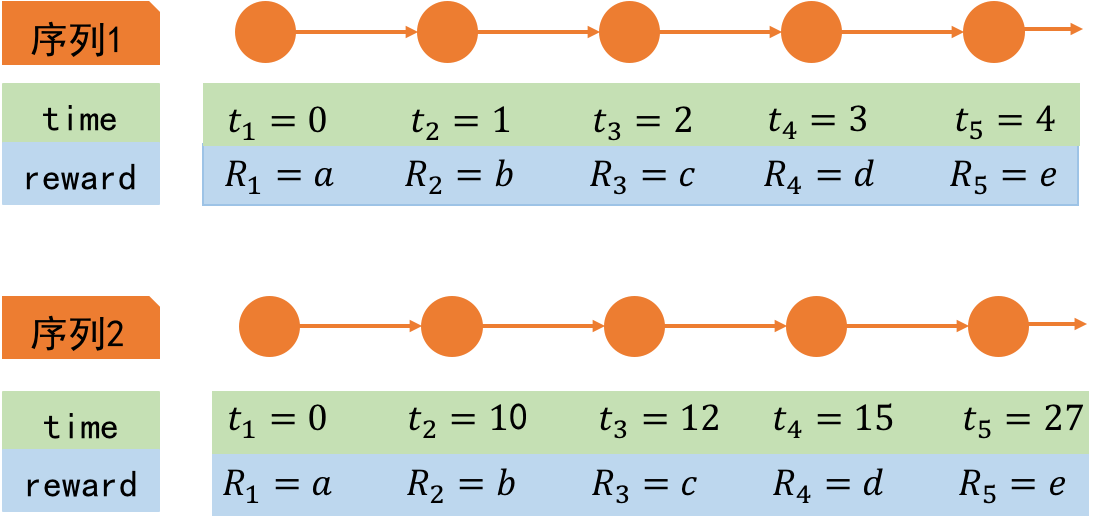
\includegraphics[width=0.8\textwidth]{2_ad_process_}
\caption{固定时间间隔序列和不固定时间间隔序列}
\label{fig:2_ad_process_}
\end{figure}

在有关马尔科夫的理论研究中,将状态逗留时间服从任意分布的决策过程称为半马尔科夫决策过程(Semi-Markov Secision Process, SMDP)\citep{guo2015survey}。SMDP中状态逗留时间不固定和上述不定期直复营场景中营销时间间隔不固定的特点十分相似.但是,不同的是在SMDP中假设时间是连续的,而在直复营销场景中时间是离散的。所以,参考SMDP问题的形式化描述,可以将时间间隔不固定的非定期直复营销问题描述为:

在时间间隔不固定的直复营销决策过程中,首先需要给每次的营销事件标记上时间,假设整个决策过程是从$t_{1}=0$时刻开始的,并且客户的初始状态为$S_{1}$,之后营销人员重复的采取营销行为,便会得到一系列的由状态、行为、奖赏以及时间组成的四元组$\{<S_{i},A_{i},R_{i},t_{i}>\}_{i=1}^{\infty}$,其中$t_{i}$是第$i$个营销事件发生的时间。那么,在计算累积折扣奖赏时,折扣因子就要被定义为关于时间的函数,如式\eqref{seq:r}所示:
\begin{equation}\label{seq:r}
\begin{aligned}
G=\sum_{i=1}^{\infty} \gamma^{t_{i}}R_{i}
\end{aligned}
\end{equation}

下面,考虑将公式\eqref{seq:r}关于累积折扣奖赏的定义结合到Q-learning算法$\ref{algo:SVR+Q}$的更新过程中。如果将第$i$个情节中的第$j$个事件和第$j-1$个事件的时间差记为:$\triangle t_{i,j} = t_{i,j}-t_{i,j-1}$。那么,利用算法$\ref{algo:SVR+Q}$中第5行对奖赏值$R_{i,j}$进行逼近后(作为初始的Q值函数),第10行的状态值的更新公式可表示为\eqref{seq:r1}:
\begin{equation}\label{seq:r1}
\begin{aligned}
v_{i,j}^{(p)}&=Q^{(p-1)}(S_{i,j},A_{i,j}) \\
&+  \alpha^{(p)} (R_{i,j} + \gamma^{\triangle t_{i,j+1}} \max_{a} Q^{(p-1)}(S_{i,j+1},a)-Q^{(p-1)}(S_{i,j},A_{i,j}))\\
% &=(1-\alpha^{(p)})Q^{(p-1)}(S_{i,j},A_{i,j}) + \alpha^{(p)} (R_{i,j} + \gamma^{\triangle t_{i,j+1}} \max_{a} Q^{(p-1)}(S_{i,j+1,},a))\;
\end{aligned}
\end{equation}

\begin{algorithm}[htbp]
\small
\SetAlgoLined
\SetKwRepeat{Repeat}{repeat}{until} 
\KwData{折扣因子$\gamma$,多项式次数$M$,最大迭代轮数$P$,原始样本集合$D=\{e_{i}|i=1,\cdots,I\}$,其中$e_{i}=\{<S_{i,j}, A_{i,j}, R_{i,j}, t_{i,j}>|j=1,\cdots,l_{i}\}$,($D_{i}$表示第$i$个渠道的样本,$e_{i,j}$表示第$i$个渠道第$j$个情节,$l_{i,j}$为$e_{i,j}$的长度)}

\KwResult{输出最终的逼近模型:$Q^{(P)}$}

\For{all $e_{i} \in D$}{
	$\triangle t_{i,1}=1$\;
	\For{$j=2$ \KwTo $l_{i}$}{

		计算时间间隔,$\triangle t_{i,j}=t_{i,j}-t_{i,j-1}$\;
	}
}
\For{all $e_{i} \in D$}{
	\For{$j=1$ \KwTo $l_{i}-1$}{
		初始的标准化因子:$\Gamma^{(0)}_{i,j}=\triangle t_{i,j}$\;
		初始的状态值:$v^{(0)}_{i,j} = R_{i,j}$\;
		将初始的状态值使用标准化因子进行标准化:$D_{i}^{(0)}=\{<S_{i,j}, A_{i,j}, \frac{v^{(0)}_{i,j}}{\Gamma^{(0)}_{i,j}}>|j=1,\cdots,l_{i}\}$\;
	}
}

同算法$\ref{algo:SVR+Q}$中第4行到第5行\;

\For{$p=1$ \KwTo $P$}{
	\For{all $e_{i} \in D$}{
		\For{$j=1$ \KwTo $l_{i}-1$}{
			更新状态行为值\;
			% $v_{i,j}^{(p)}=(1-\alpha^{(p)})Q^{(p-1)}(S_{i,j},A_{i,j}) \cdot \triangle  Z_{i,j}^{(p-1)} 
			% + \alpha^{(p)} (R_{i,j} + \gamma^{\triangle t_{i,j+1}} \max_{a} Q^{(p-1)}(S_{i,j+1,},a) \cdot \triangle  Z_{i,j+1}^{(p-1)} )$\;
			$v_{i,j}^{(p)}=Q^{(p-1)}(S_{i,j},A_{i,j}) \cdot  \Gamma_{i,j}^{(p-1)}
			+  \alpha^{(p)} (R_{i,j} + \gamma^{\triangle t_{i,j+1}} \max_{a} Q^{(p-1)}(S_{i,j+1},a) \cdot \Gamma_{i,j+1}^{(p-1)} -Q^{(p-1)}(S_{i,j},A_{i,j}) \cdot  \Gamma_{i,j}^{(p-1)} )$\;

			更新标准化因子\;
			% $Z^{(p)}_{i,j}=(1-\alpha^{(p)})Z^{(p-1)}_{i,j}+\alpha^{(p)}(\triangle t_{i,j+1} + \gamma^{\triangle t_{i,j+1}} \cdot Z^{(p-1)}_{i,j+1})$\;
			$\Gamma^{(p)}_{i,j}=\Gamma^{(p-1)}_{i,j}+\alpha^{(p)}(\triangle t_{i,j+1} + \gamma^{\triangle t_{i,j+1}} \cdot \Gamma^{(p-1)}_{i,j+1}-\Gamma^{(p-1)}_{i,j})$\;
		}
		更新第$i$个情节的样本:$D_{i}^{(p)}=\{<S_{i,j}, A_{i,j}, \frac{v_{i,j}^{(p)}}{\Gamma^{(p)}_{i,j}}>|j=1,\cdots,l_{i}-1\}$\;
	}
	同算法$\ref{algo:SVR+Q}$中第14行到第15行\;
}
输出最终的Q值函数$Q^{(P)} = Q^{(P)} \cdot \Gamma^{(P)}$\;
\caption{基于Interval-Q算法的直复营销模型}
\label{algo:RBF-SVR-Q-t}
\end{algorithm}

虽然公式\eqref{seq:r1}在更新状态值$v_{i,j}$的时候考虑到了时间间隔不固定的因素($\gamma^{\triangle t_{i,j+1}}$),但是,由于算法$\ref{algo:SVR+Q}$中第5行在利用奖赏值$R_{i,j}$逼近初始的Q值函数的时候,并没有考虑到时间间隔不固定的问题,所以如果按照上述方法逼近Q值函数,并将其应用于公式\eqref{seq:r1}进行状态值的计算更新时会造成很大的偏差。所以,接下来就要寻找一种合适的Q值函数逼近方法。

如上文所述,造成Q值函数逼近不准确的原因是相邻两个决策点间的时间间隔不固定,所以一个自然的想法是利用标准化的思想,将序列中所有的时间间隔都切割成若干个固定单位的时间间隔,然后再进行Q值函数的逼近,进而再按照公式\eqref{seq:r1}更新状态值,就可以缓解因为时间间隔不同而造成的Q值函数逼近不准确的问题。具体的做法是:将时间间隔$\triangle t_{i,j}$内获得的奖赏值进行均值标准化,然后再使用标准化后的值进行Q值函数的逼近。均值标准化的公式如\eqref{seq:r_1}所示:
\begin{equation}\label{seq:r_1}
\begin{aligned}
R_{i, j}^{'}=\frac{R_{i,j}}{t_{i,j}-t_{j-1}}=\frac{R_{i,j}}{\triangle t_{i,j}}
\end{aligned}
\end{equation}

那么,此时算法$\ref{algo:SVR+Q}$中第10行的更新公式就可以按照下式\eqref{seq:r_2}的方式进行更新:
\begin{equation}\label{seq:r_2}
\begin{aligned}
% v_{i,j}^{(p)}=&(1-\alpha^{(p)})Q^{(p-1)}(S_{i,j},A_{i,j}) \cdot \triangle t_{i,j} \\
% &+ \alpha^{(p)} (R_{i,j} + \gamma^{\triangle t_{i,j+1}} \max_{a} Q^{(p-1)}(S_{i,j+1,},a) \cdot \triangle t_{i,j+1})\\
v_{i,j}^{(p)}&=Q^{(p-1)}(S_{i,j},A_{i,j}) \cdot \triangle t_{i,j} \\
&+  \alpha^{(p)} (R_{i,j} + \gamma^{\triangle t_{i,j+1}} \max_{a} Q^{(p-1)}(S_{i,j+1},a) \cdot \triangle t_{i,j+1} -Q^{(p-1)}(S_{i,j},A_{i,j}) \cdot \triangle t_{i,j} )\\
\end{aligned}
\end{equation}

接着,按照算法$\ref{algo:SVR+Q}$中第12行进行情节样本的更新:
\begin{equation}\label{seq:r_3}
\begin{aligned}
D_{i}^{(p)}=\{<S_{i,j}, A_{i,j}, \frac{v_{i,j}^{(p)}}{\triangle t_{i,j}}>|j=1,\cdots,l_{i}-1\}\;
\end{aligned}
\end{equation}

但是,从公式\eqref{seq:r_2}中可以看出,随着迭代轮数的增加,$v_{i,j}$在不断变化,而$\triangle t_{i,j}$是始终不变的,所以,如果一直按照公式\eqref{seq:r_3}中状态值的更新方式($\frac{v_{i,j}^{(p)}}{\triangle t_{i,j}}$)进行样本情节的更新,就会因为这两个值的更新不同步而给值函数的学习带来一定的偏差。因此,本文的想法是,在状态值的更新过程中,应该仿照$v_{i,j}$的更新方式进行$\triangle t_{i,j}$的更新。针对这个问题,本文基于时间间隔构建一个标准化因子$\Gamma_{i,j}$,并仿照$v_{i,j}$的更新方式进行标准化因子的更新,以减少偏差带来的影响。标准化因子的更新方式可表示为式\eqref{seq:r_5}的形式:

\begin{equation}\label{seq:r_5}
\begin{aligned}
% Z^{(p)}_{i,j}=(1-\alpha^{(p)})Z^{(p-1)}_{i,j}+\alpha^{(p)}(\triangle t_{i,j+1} + \gamma^{\triangle t_{i,j+1}} \cdot Z^{(p-1)}_{i,j+1})\\
\Gamma^{(p)}_{i,j}=\Gamma^{(p-1)}_{i,j}+\alpha^{(p)}(\triangle t_{i,j+1} + \gamma^{\triangle t_{i,j+1}} \cdot \Gamma^{(p-1)}_{i,j+1}-\Gamma^{(p-1)}_{i,j})\;
\end{aligned}
\end{equation}

由此,可以得到基于时间间隔不固定的Q-learning算法如$\ref{algo:RBF-SVR-Q-t}$所示,记为Interval-Q。其中,第1行到第6行进行时间间隔的计算,第7行到第13行进行标准化因子以及样本的的初始化,第19行进行状态行为值的更新,第21行进行归一化因子的更新,第23进行情节样本的更新。

\subsection{基于TD偏差的Q采样算法}
在像直复营销这种现实的应用场景中,每天面对的数据量非常大,如果将全部样本都导入模型中进行训练,将必然会加重模型的训练负担消耗很多的训练时间。另外,训练样本中不同样本有着不同的学习效率,有的样本甚至会影响模型的训练效果。所以,针对以上问题,应该采取有效的采样方法来加快模型的训练,以提高值函数的学习效率。

在强化学习中,常用的采样方法有随机采样法\citep{tsitsiklis1994asynchronous}和Q采样法\citep{abe2002empirical}。随机采样法,就是在每次从数据集中取情节的时候(如算法$\ref{algo:RBF-SVR-Q-t}$中,第7行和第16行),并不是取所有的情节,而是随机选取部分的情节。这种随机采样方法虽然可以减少模型的训练和更新时间,但是由于随机性较高,导致采样后的数据质量并不高,因而会影响最后值函数的逼近效果。Q采样法,是在随机采样的基础上利用Q-learning的更新策略提出的,当进行Q值函数进行更新的时候,不是每个情节中所有事件都会被选择用于值函数的更新,而只有那些利用当前的估计Q值函数,可以在下一个状态中取得最佳行为的状态才能被选择。即将算法$\ref{algo:RBF-SVR-Q-t}$的第16到24行替换成如下算法$\ref{algo:SVR+Q_}$的语句:

\begin{algorithm}[htbp]
\small
\SetAlgoLined
\SetKwIF{If}{ElseIf}{Else}{if}{then}{else if}{else}{endif}
从数据集合$D$中随机采样一个样本子集,$B^{(p)}$\;
\For{all $e_{i} \in B^{(p)}$}{
	\For{$j$ \KwTo $l_{i}-1$}{
		\If{$Q^{(p-1)}(S_{i,j+1},A_{i,j+1})=\max_{a}Q^{(p-1)}(S_{i,j+1},a)$}{

			$v_{i,j}^{(p)}=Q^{(p-1)}(S_{i,j},A_{i,j}) \cdot  \Gamma_{i,j}^{(p-1)}
			+  \alpha^{(p)} (R_{i,j} + \gamma^{\triangle t_{i,j+1}} Q^{(p-1)}(S_{i,j+1},A_{i,j+1}) \cdot \Gamma_{i,j+1}^{(p-1)} -Q^{(p-1)}(S_{i,j},A_{i,j}) \cdot  \Gamma_{i,j}^{(p-1)} )$\;

			$\Gamma^{(p)}_{i,j}=\Gamma^{(p-1)}_{i,j}+\alpha^{(p)}(\triangle t_{i,j+1} + \gamma^{\triangle t_{i,j+1}} \cdot \Gamma^{(p-1)}_{i,j+1}-\Gamma^{(p-1)}_{i,j})$\;
		}
		更新第$i$个情节的样本:$D_{i}^{(p)}=D_{i}^{(p)} \cup \{<S_{i,j}, A_{i,j}, \frac{v_{i,j}^{(p)}}{\Gamma^{(p)}_{i,j}}>\}$\;
	}
}
\caption{基于Q采样的算法}
\label{algo:SVR+Q_}
\end{algorithm}

但是,通过Q采样的方法进行采样后的样本仍然很大,而且,即使选择了在下一状态中可以达到最佳行为的当前状态,但是该状态并不一定会有很高的学习效率。考虑在本文第二章中,由公式$\eqref{shijiachafen}$计算出的$t$时刻的时间差分TD:$\delta_{t}$,应用在算法$\ref{algo:SVR+Q_}$的Q值函数中,可表示为式$\eqref{shijiachafenq}$:
\begin{equation}\label{shijiachafenq}
\begin{aligned}
&\delta_{i,j}=R_{i,j} + \gamma^{\triangle t_{i,j+1}} Q^{(p-1)}(S_{i,j+1}, a) \cdot \Gamma_{i,j+1}^{(p-1)}  - Q^{(p-1)}(S_{i,j},A_{i,j}) \cdot \Gamma_{i,j}^{(p-1)} \\
&\text{其中,} a=\argmax_{a} (Q^{(p-1)}(S_{i,j+1},a) \cdot \Gamma_{i,j+1}^{(p-1)})
\end{aligned}
\end{equation}

在式$\eqref{shijiachafenq}$中,$R_{i,j} + \gamma^{\triangle t_{i,j+1}} Q^{(p-1)}(S_{i,j+1}, a) \cdot \Gamma_{i,j+1}^{(p-1)}$称为TD目标,即值函数逼近的目标值。如果TD偏差$\delta_{t}$越大,说明该状态处的值函数$Q^{(p-1)}(S_{i,j},A_{i,j}) \cdot \Gamma_{i,j}^{(p-1)}$与TD目标的差距越大,进一步可以说明Agent的更新量越大,因此在该处的学习效率就越高。所以,TD偏差其实可以作为是评价样本学习效果的一个指标。基于这个想法,在进行Q采样的时候,可以根据TD偏差进行约束。具体地,当使用Q采样算法$\ref{algo:SVR+Q_}$第4行条件进行初步选择后,设定一个固定的阈值$\eta$,然后使用公式$\eqref{shijiachafenq}$再一次进行选择,只选择TD偏差大于$\eta$的样本进行更新。所以,基于这个想法就可以得到基于TD偏差的Q采样法如算法$\ref{algo:SVR+Q_2}$所示。在实际应用中,对于阈值$\eta$的选取可以从训练样本的奖赏均值附近处开始尝试,通过观察采样数和策略学习效果再进一步确定。

\begin{algorithm}[htbp]
\small
\SetAlgoLined
\SetKwIF{If}{ElseIf}{Else}{if}{then}{else if}{else}{endif}
\KwData{增加一个TD偏差阈值$\eta$}
从数据集合$D$中随机采样一个样本子集,$B^{(p)}$\;
\For{all $e_{i} \in B^{(p)}$}{
	\For{$j$ \KwTo $l_{i}-1$}{
			利用公式$\eqref{shijiachafenq}$计算的$\delta_{i,j}$\;
		\If{$Q^{(p-1)}(S_{i,j+1},A_{i,j+1})=\max_{a}Q^{(p-1)}(S_{i,j+1},a)$ $\bm{And}$
			$\delta_{i,j} \geqslant$  $\eta$
		}{
			$v_{i,j}^{(p)}=Q^{(p-1)}(S_{i,j},A_{i,j}) \cdot  \Gamma_{i,j}^{(p-1)}
			+  \alpha^{(p)} (R_{i,j} + \gamma^{\triangle t_{i,j+1}} Q^{(p-1)}(S_{i,j+1},A_{i,j+1}) \cdot \Gamma_{i,j+1}^{(p-1)} -Q^{(p-1)}(S_{i,j},A_{i,j}) \cdot  \Gamma_{i,j}^{(p-1)} )$\;

			$\Gamma^{(p)}_{i,j}=\Gamma^{(p-1)}_{i,j}+\alpha^{(p)}(\triangle t_{i,j+1} + \gamma^{\triangle t_{i,j+1}} \cdot \Gamma^{(p-1)}_{i,j+1}-\Gamma^{(p-1)}_{i,j})$\;
		}
		更新第$i$个情节的样本:$D_{i}^{(p)}=D_{i}^{(p)} \cup \{<S_{i,j}, A_{i,j}, \frac{v_{i,j}^{(p)}}{\Gamma^{(p)}_{i,j}}>\}$\;
	}
}
\caption{基于TD偏差的Q采样算法}
\label{algo:SVR+Q_2}
\end{algorithm}

\section{仿真实验}
本节,将借助直复营销场景中的直邮营销数据进行模型的训练,并通过仿真的方法进行模型的评估。首先,对实验中所使用的数据集进行介绍,并详细说明所选择的客户状态特征;然后,介绍本实验中的仿真环境构建方法和模型效果的评估方法;接着,描述本章实验用到的基准模型以及相关实验设置信息;最后,从模型所产生的长期利润、策略行为的变化情况以及不同采样方法的效果对比等三方面对模型进行评估并对结果进行分析。

\subsection{数据集}
本章的试验数据集选择使用UCI机器学习数据库中关于直邮营销著名的公开数据集KDD-CUP 1998\footnote{https://archive.ics.uci.edu/ml/datasets/KDD+Cup+1998+Data.html}。该数据集有两个用途,一方面,利用数据集中的数据训练模型,以生成最优的营销策略。另一方面,利用该数据集构建基于马尔科夫决策过程的仿真环境,然后利用这个仿真模型进行仿真实验,以评估不同模型所生成的营销策略。

\paragraph{数据集背景}
直邮营销是直复营销中最早的、也是最为经典的营销形式,它通过对目标客户以邮寄的方式达到营销宣传的目的。KDD-CUP 1998数据集是由美国非盈利组织PVA(Paralyzed Veterans of America)收集的,该组织通过直邮的方式向潜在的捐助者发布募捐活动信息以
筹集资金,为有脊髓损伤疾病的美国退伍军人提供医疗资金援助。

该数据集由PVA组织在两年间对95412名捐助者进行募捐营销的历史营销纪录所组成,一共包含22次连续的募捐活动,每个募捐活动之间的时间间隔为0-3个月不等。该数据集中每个捐助者的信息由481维数据组成,这些数据可以概括为以下三个方面的信息:

(a)捐助者的全面人口统计数据,包括家庭和所在地区两个层面的组合数据:比如:捐助者的年龄、收入、性别、家庭信息以及该捐助者所在地区的相关信息等,共计361维。

(b)两年间所进行的22次募捐活动的营销与反馈数据。比如:PVA在每一次的营销活动中是否向该捐助者进行了邮寄营销、进行邮件营销的时间、捐助者是否对PVA的每一次邮件营销产生了捐助反馈、募捐的金额以及募捐的时间,以及在每一次捐助活动时捐助者的RFA( Recency/Frequency/Amount, 距离最后一次募捐的时间/到目前为止募捐的频率/上一次募捐的总额)状态值等信息 ,共计99维,其中募捐的金额从0-1000美元不等。

(c)在最后一次募捐营销结束后每个捐助者的概括信息(Summary Variables)。比如:迄今(最后一次募捐结束后)为止该捐助者捐助的总金额、迄今为止该捐助者捐助的总次数、迄今为止PVA对该捐助者开展邮件营销的总次数以及迄今为止该捐助者所捐助过的最大金额等信息,共计21维。

有关该数据集的其它描述信息可在UCI网站上获得。因为原始数据集中涉及了大量的用户特征,但是在本章实验中只选取了部分特征,所以在本章的后续部分再对所使用的数据特征进行详细介绍。

\begin{table}[htbp]
  \centering
  \caption{捐助者的状态特征}
  \label{tab:obser_donors}
  \begin{tabular}{lll}
    \toprule
      序号 & 特征 & 描述 \\
    \midrule
      1 & age & 捐助者的年龄 \\
      2 &income & 捐助者的收入 \\
      3 &ngiftall & 到目前为止,捐助者捐助的次数 \\
      4 &numprom & 到目前为止,PVA向该捐者发送直邮营销的次数 \\
      5 &frequency & 到目前为止,该捐助者捐助的频率:ngiftall / numprom \\
      6 &ramntall & 到目前为止,捐助的总金额 \\
      7 &recency & 距离上次捐助的时间 \\
      8 &promrecency & 距离上次发送直邮营销的时间\\
      9 &timelag & 第一次直邮营销和第一次捐助的时间\\
      10 &recencyratio & recency / timelag\\
	  11 &promrecratio & promrecency / timelag\\
      12 &nrecproms6 & 之前六个月里,给该捐者者发送直邮营销的次数\\
      13 &nrecgifts6 & 之前六个月里,捐助者捐助的次数\\
      14 &totrecamt6 & 之前六个月里,捐助者捐助的金额之和\\ 
      15 &nrecproms3 & 之前三个月里,给该捐者者发送直邮营销的次数\\
      16 &nrecgifts3 & 之前三个月里,捐助者捐助的次数\\
      17 &totrecamt3 & 之前三个月里,捐助者捐助的金额之和\\            	  
	  % 18 &action & PVA的营销类型,0表示未进行,1表示已进行\\
	  % 19 &money &  捐助的金额\\
    \bottomrule
  \end{tabular}
\end{table}

\paragraph{数据处理与特征选择}
首先,需要确定算法中的数据结构。在算法$\ref{algo:RBF-SVR-Q-t}$中,数据是以情节(episode)的形式存在的,每个情节内又包含一系列有序的事件(event),每个事件是由状态,行为、奖赏和时间所构成的四元组。因此,在KDD-CUP 1998数据集中,可以将每个捐助者的22次营销数据序列看作一个情节,每一次的营销看作情节中的一个事件。那么,每个捐助者就对应一个情节,每个情节里有22个事件,且22个事件是按照真实的营销时间有序排开的。特别地,每个事件里包括该捐助者当时的状态特征,PVA对其采取的营销行为、此次营销捐助的金额以及该营销活动所发生的时间。

为了能够准确地描述捐助者在每一次营销活动中的状态,通常需要借助专家领域知识,选取高效的用户特征。本节主要参考文献\citep{tkachenko2015autonomous, pednault2002sequential}中客户特征的选取方法,从KDD-CUP 1998数据集中提取募捐者的状态特征。具体地,针对每个捐助者的个人基本信息,本章只选择了年龄和收入两个指标,此外,根据数据集中募捐者的历史营销记录,生成了许多临时特征,以更好的捕捉募捐者的近期状态,如表~\ref{tab:obser_donors}所示。从表~\ref{tab:obser_donors}中可以看到,本节使用了一个六个月的历史时间窗口和一个三个月的历史时间窗口来提取捐助者的近期状态特征,所以,数据库中最开始的六个月数据就被用于构建第一个历史窗口信息了,那么,一个情节中的22个事件就只剩下16个左右可以用于模型的训练了。

需要注意的是,在表~\ref{tab:obser_donors}中,捐助者的大部分状态特征都无法从数据集中直接获得,而只能通过遍历数据库进行统计、计算而得到。比如,在数据集中,每个捐助者的numprom字段只有一个值,它表示的意思是最后一次营销(第22次)结束后向该捐助者发送直邮营销的次数 ,那么为了得到之前21次营销活动中该捐助者的numprom值,应该按照营销活动的顺序从后往前进行遍历,每当在数据集中发现PVA对该捐助者进行了邮寄,就进行减一操作。同样,对于ngiftall字段,在数据集中每个捐助者也只有一个值,它表示的意思是最后一次营销结束后该捐助者一共捐助的次数,而为了得到之前21次营销活动中该捐助者的ngiftall值,应该按照营销活动的顺序从后往前进行遍历,每当在营销活动中发现该捐助者进行了捐助就进行减一操作。按照上述方式就可以得到在每次营销活动时捐助者的ngiftall和numprom值了,那么捐助者的frequency也就可以求出来了。同样地,表~\ref{tab:obser_donors}中的其他特征也可以按照这种方式求得。

另外,算法\ref{algo:RBF-SVR-Q-t}中的行为(action)对应PVA的营销类型,0表示未进行直邮营销,1表示已进行直邮营销;算法中的奖赏(reward)信息对应PVA所获得的募捐利润值。

\subsection{仿真环境及评估方法}
因为强化学习算法主要用于解决序贯决策问题,所以评估强化学习模型的好坏需要有稳定的仿真环境。目前,OPENAI\footnote{https://openai.com/}提供了许多游戏的仿真环境开源库,科研人员可以通过其提供的API接口非常方便的调用这些仿真环境,来训练、测试自己的模型,因此,这也是目前大多数强化学习的研究者选择在游戏领域进行研究的一个重要原因。然而,在其它的一些现实应用中,需要研究人员根据数据集自己构建仿真环境。在本节,利用KDD-CUP 1998数据集,按照文献\citep{pednault2002sequential}中提供的方法,通过构建关于募捐者的马尔科夫决策过程模型来搭建仿真环境,进而评价模型输出策略的好坏。

\paragraph{构建MDP模型}
马尔科夫决策过程主要由两个模型组成:第一个模型$P(s,a)$是用来预测捐助者的产生募捐反馈的响应概率,它是一个关于状态$s$和行为$a$的函数。第二个模型$A(s,a)$用来预测如果募捐者对此次募捐邮件产生了响应,会产生多少金额的捐款。在本节的实验中模型$P(s,a)$和$A(s,a)$分别使用随机森林分类模型和随机森林回归模型进行构建。

当有了模型$P(s,a)$和$A(s,a)$就可以使用如下过程来构建马尔科夫决策过程了。(如图$\ref{fig:simulation}$中“仿真环境模块”所示)

(a)给定状态$s$和行为$a$下的即时利润$R(s,a)$可以通过以上这两个模型得到:以$P(s,a)$的概率来掷一枚硬币,并以此来判断捐助者是否会产生反馈。即:出现正面的概率为$P(s,a)$表示捐助者会产生反馈,出现反面的概率为$1-P(s,a)$表示捐助者忽略掉了本次募捐邮件,不会产生任何反馈信息。如果没有出现反馈,那么捐助额为$0$,如果产生了反馈,那么用户的捐助金额为$A(s,a)$。即时利润$R(s,a)$等于捐助额减去邮寄的成本。

(b)状态转移方程也可以使用上述这两个模型通过独立地计算每一维状态特征的变化值而得到。比如:如果PVA采取的行动为1(进行邮寄营销),numprom的值就会加1,否则保持不变;同样的,如果通过上述方式投掷的硬币出现正面朝上,那么ngiftall的值就会加1,否则保持不变;有了这两个值(numprom,ngiftall),那么frequency的值也就可以计算出来了。类似的,其他状态特征也是通过这种方法计算得到的。

\begin{figure}[htbp]
\centering
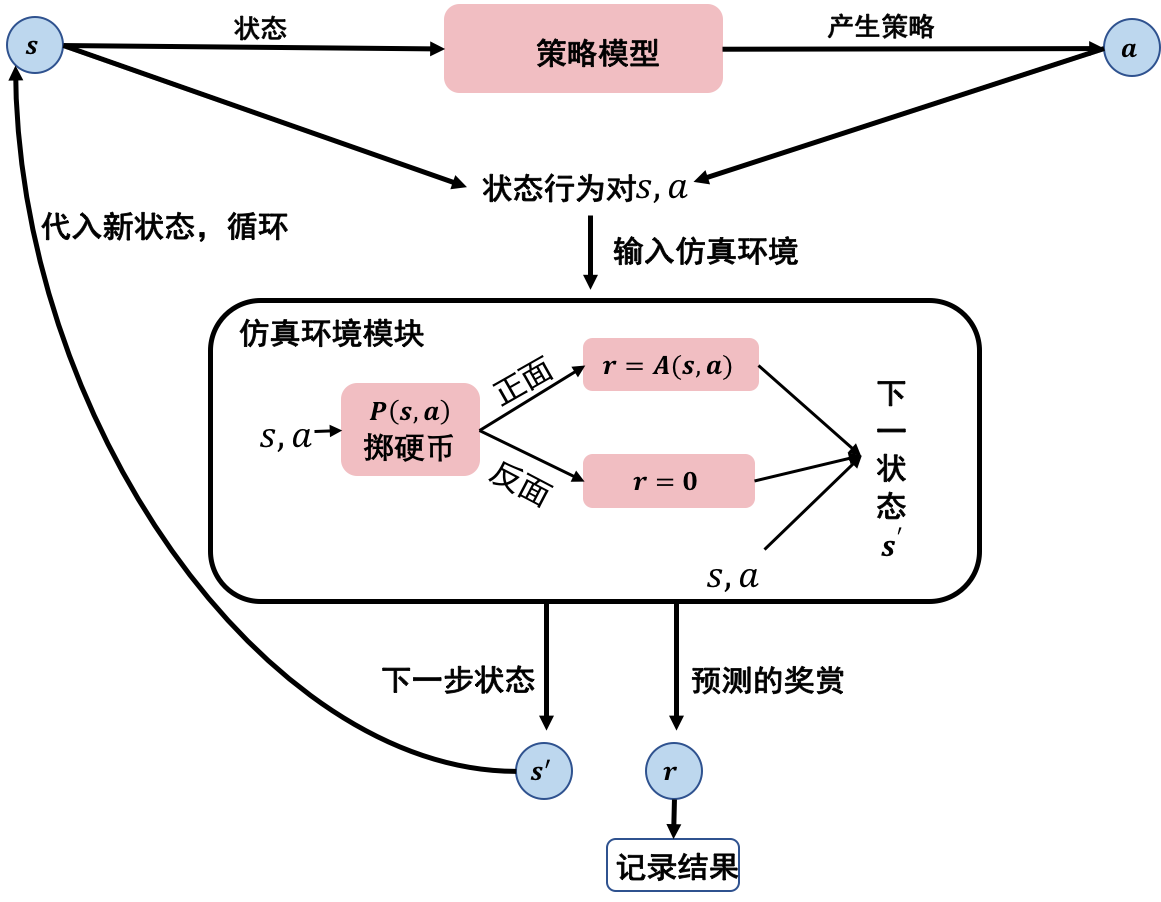
\includegraphics[width=0.8\textwidth]{simulation}
\caption{仿真评估实验流程图}
\label{fig:simulation}
\end{figure}

\paragraph{评估方法}
如图$\ref{fig:simulation}$所示,有了上述基于马尔科夫决策过程的模型和状态转移方程,就可以使用如下的方式来评估实验。

(a)首先,从数据集中随机选择一定数量的捐助者,并设置他们的初始状态$s$。

(b)然后,使用训练好的强化学习模型输出营销策略:对每个捐助者是否应该采取营销行为$a$。

(c)最后,将状态$s$和策略行为$a$代入仿真环境中,使用模型$P(s,a)$和$A(s,a)$,就可以得到预估的即时奖赏$r$以及下一时刻的状态$s^{'}$。记录这些得到信息,然后进入下一次的邮寄决策中。

此后,按照上述的三个步骤,每循环一次就会模拟一次虚拟的直邮营销过程。在本节实验中,重复循环了20次,就得到了20次的虚拟直邮营销数据,通过计算每个模型策略在20次虚拟营销中的长期利润,进而评价模型策略的好坏。

在文献\citep{pednault2002sequential}中作者提出,构建上述仿真环境的前提假设是认为募捐者的交互过程是一个马尔科夫决策过程,但是,在现实中这不一定是合适的。作者认为,像直复营销这种与人类行为有关的场景都过于复杂,使用简单的马尔科夫决策过程是无法较好地捕捉到环境的变化规律的。但是,就像在本章中,通过这种方法设计的仿真环境只是去评估模型所产生的策略的好坏,只是在真实场景应用前的一个评估实验。因此,这种评估方法是可接受的,也是目前强化学习评估实验所普遍采用的方法。

\subsection{基准模型与实验设置}
\paragraph{基准模型}
在本节一共选择四个基准模型来验证上述两个改进的算法,其中Interval-Q算法的对照基准模型包括:多项式回归模型以及Batch Q-learning算法\citep{pednault2002sequential}。基于TD偏差的Q采样算法的基准模型包括:随机采样法和Q采样法。因为随机采样法和Q采样法在本章第二节的内容都有介绍,所以下面只介绍Interval-Q算法的基准模型。

监督模型:多项式回归模型。为了比较监督学习和非监督学习在序列决策问题中的差异,考虑使用监督学习方法作为基准模型。另外,因为在Interval-Q算法中,函数逼近模型采用的是多项式回归模型,所以,为了公平起见,此处仍然选用多项式回归模型作为对照的监督学习模型。在训练模型时,只要将算法$\ref{algo:SVR+Q}$中的$P$设置为0即可,即基于状态$s$和行为$a$来预测即时利润$r$,将学到的模型记为$\hat{R}(s,a)$。当模型训练好后,将募捐者的状态$S_{t}$带入模型$\hat{R}(s,a)$中来估计进行营销时所能获得的即时利润,如果即时利润不为负,则发送营销邮件,否则不发送。

强化学习模型:Batch Q-learning算法。通过此算法来比较引入时间间隔不固定的因素后对模型策略效果所产生的影响。


\paragraph{实验设置}
(a)所有实验运行在Mac Pro机器上,内存16GB,实验语言:Python,机器学习工具包:scikit-learn。

(b)本节试验中,每个模型在相同的参数设置下,分别进行5次试验,每次实验最大迭代轮数$P$为8轮(包括第0轮,其实一共迭代了9轮)。每一轮迭代结束后输出模型所产生的营销策略并按照上述方法使用仿真环境评估该策略,最后取5次实验中每一轮迭代的平均值作为该模型该轮迭代的结果。另外,测试的样本规模大小为5000,并设置他们的初值状态为数据库中对应第7次营销活动时的状态。

(c)在所有的强化学习方法中,衰减因子设为$\gamma=0.9$,通过交叉验证法确定多项式最高次数为5。

% (d)在使用随机森林构建仿真环境时,通过网格搜索法确定以下参数:最大的弱学习器的个数为115个,决策树最大深度为25,叶子节点最少样本数为3,其它参数均选择sklearn的默认值。

\subsection{仿真结果}
下面,本节将从模型策略的长期利润、策略行为的变化情况以及不同采样方法的效果对比等三方面展开对模型的评估与分析。具体地,从模型在20次虚拟营销中所获得的累积总利润、策略行为的变化情况来比较Interval-Q算法、Batch Q-learning算法以及多项式回归算法策略的质量。从模型训练时事件的采样数以及该采样数下所产生的长期利润这两个角度来比较基于TD偏差的Q采样法、Q采样法以及随机采样法的性能。

\paragraph{长期利润}
首先,考察Interval-Q算法,Batch Q-learning算法以及多项式回归模型在20个虚拟营销中的累积总收益,即长期利润。在该实验中,每次实验都随机选取10000个用户的历史营销纪录,也就是10000个情节数据进行训练,每进行完一轮迭代就按照上述方法利用仿真环境进行评估测试,评估模型此时的营销策略在20个虚拟营销中的总利润,并将每一次迭代所产生的结果记录下来。其中,测试集的样本大小为5000。

\begin{table}[htbp]
\centering
\footnotesize
\caption{Interval-Q算法的长期利润(单位:百美元)}
\label{tab:3result1}
\begin{tabular}{|c|ccccccccc|}  
 % \toprule
 \hline
   \diagbox{试验次数}{迭代数} &0 & 1&2 &3 &4 &5 &6 &7 &8\\
% \midrule
\hline

第一次 &5123	&5299	&5557	&5723	&5847	&5854	&5867	&5864	&5868\\
第二次 &5224	&5339	&5666	&5811	&5908	&5911	&5921	&5926	&5920\\
第三次 &5262	&5404	&5602	&5843	&5984	&5981	&5996	&6013	&6015\\
第四次 &5102	&5324	&5569	&5711	&5792	&5888	&5905	&5907	&5917\\
第五次 &5181	&5333	&5602	&5813	&5968	&5971	&5987	&5985	&5987\\
\hline
平均值 &5178	&5340	&5599&5780	&5890	&5921	&5935	&5939&	5941\\
\hline
标准差 &	&17	&17	&18	&33	&22&22	&25	&24\\
% \bottomrule
\hline
\end{tabular}
\end{table}

\begin{table}[htbp]
\centering
\footnotesize
\caption{Batch Q-learning算法的长期利润(单位:百美元)}
\label{tab:3result2}
\begin{tabular}{|c|ccccccccc|}  
 % \toprule
 \hline
  \diagbox{试验次数}{迭代数} & 0 & 1&2 &3 &4 &5 &6 &7 &8\\
% \midrule
\hline
第一次 &5123	&5234&	5586&	5735&	5797&	5814&	5798&	5795&	5801\\
第二次 &5224	&5322&	5659&	5786&	5841&	5883&	5887&	5897&	5870\\
第三次 &5262	&5453&	5655&	5806&	5869&	5927&	5935&	5929&	5936\\
第四次 &5102	&5358&	5578&	5601&	5659&	5679&	5710&	5707&	5713\\
第五次 &5181	&5499&	5698&	5781&	5862&	5918&	5926&	5937&	5936\\
\hline
平均值 &5178	&5373&	5635&	5742	&5806&	5844&	5851&	5853&	5851\\
\hline
标准差 &	&	43	&21	&34	&35	&42	&39	&41&	39\\
% \bottomrule
\hline
\end{tabular}
\end{table}

表~\ref{tab:3result1}和表~\ref{tab:3result2}分别展示了Interval-Q算法、Batch Q-learning算法在这5次试验中的每一轮迭代结束后各模型策略所产生的长期利润值。其中,两个表中第0轮迭代的结果是指多项式回归模型策略的在20个虚拟营销中的总利润,表中标准差的计算方式如式\eqref{seq:shiyan_2}所示。
\begin{equation}\label{seq:shiyan_2}
\begin{aligned}
\sigma = \sqrt{\frac{\sum_{i=1}^{n}(F_{i}-\bar{F})^{2}/n-1}{n}}
\end{aligned}
\end{equation}

在式$\eqref{seq:shiyan_2}$中,$F_{i}$表示在第$i$轮迭代中的总收益,$\bar{F}$表示5次迭代中的平均收益,$n$表示试验的次数,此处为5。

为了方便观察,将表~\ref{tab:3result1}和表~\ref{tab:3result2}中的平均值画在折线图上,如图\ref{fig:e31}所示。从图\ref{fig:e31}中可以看出,Interval-Q算法和Batch Q-learning算法的营销策略在20次虚拟营销中的总利润明显大于多项式回归算法营销策略的总利润,这是因为强化学习算法在求解序贯决策问题时,考虑到了序列中的延迟影响,并且以长期收益最大化作为学习目标,而多项式回归算法在学习时,只考虑了独立事件的即时利润最大化,因此在序贯决策问题时相比强化学习方法有很大的局限性。

另外,从Interval-Q算法和Batch Q-learning算法的迭代过程中可以看出,随着迭代轮数的增长,Interval-Q算法在第3轮迭代后产生的总利润超过了Batch Q-learning算法的总利润,并且在最后一轮迭代时Interval-Q算法产生的长期利润比Batch Q-learning算法的长期利润提高了约1.54\%。这是因为Interval-Q算法在更新时考虑到了营销时间间隔不固定的问题,而Batch Q-learning算法忽视了这种情况,从而会给积累奖赏的计算带来噪声影响,进而会给值函数评估造成偏差,导致学习到的营销策略较差。另外,经计算,Batch Q-learning算法在8轮迭代中标准差的平均值为37大于Interval-Q算法在8轮迭代种的标准差的平均值22,因而说明了在时间间隔不固定的问题中,Interval-Q算法比Batch Q-learning算法输出营销策略时的稳定性更好。至此,可以证明本章的Interval-Q算法在解决时间间隔不固定问题上是有效的。

% 一方面证明强化学习的方法比监督学习的方法在序列化决策问题上会有更好的收益,另一方面期望证明基于可变时间间隔的ntervalQ模型在直复营销场景中比普通batch Q-learning模型有更好的表现。
\begin{figure}[htbp]
\centering
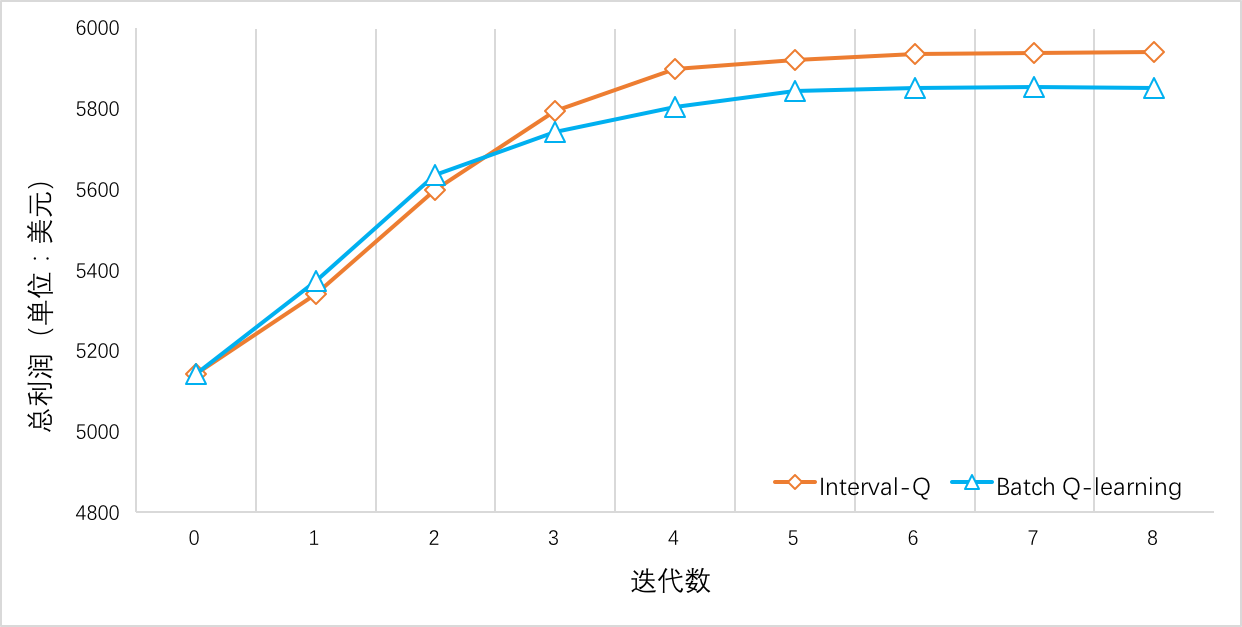
\includegraphics[width=1.0\textwidth]{e31}
\caption{Interval-Q算法和Batch Q-learning算法的总利润}
\label{fig:e31}
\end{figure}

\begin{figure}[htbp]
\centering
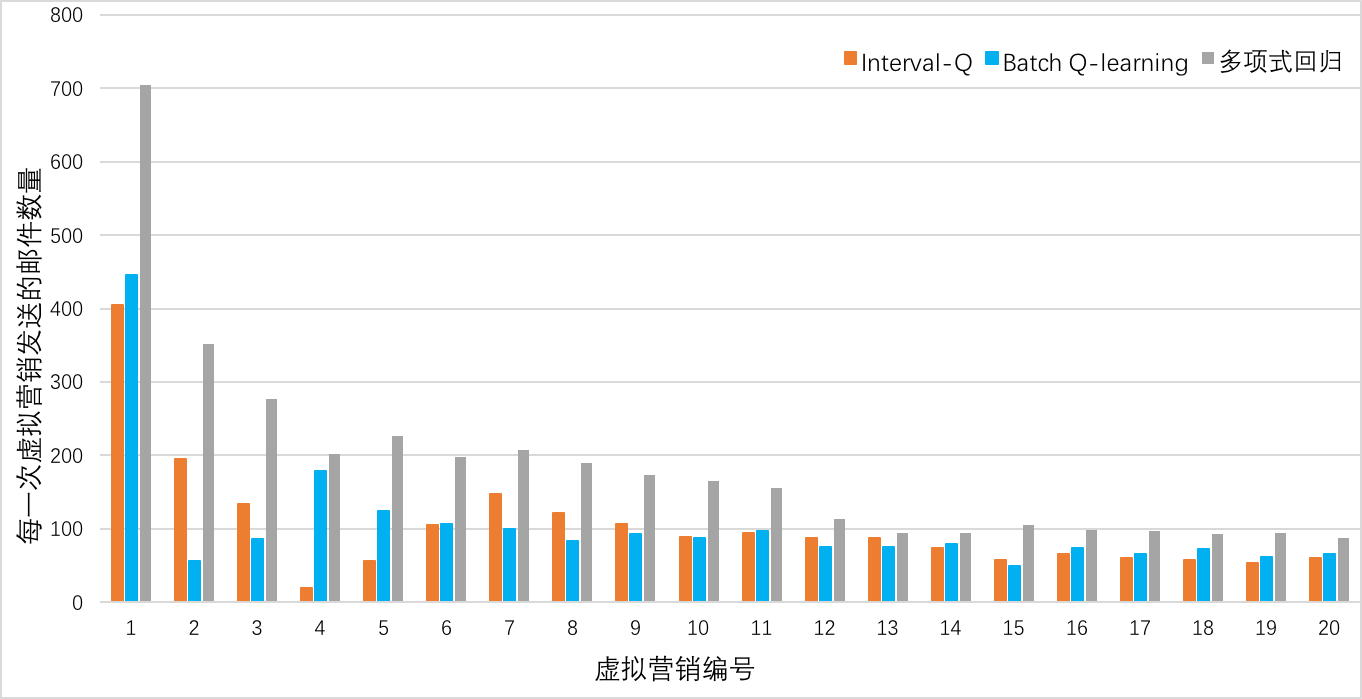
\includegraphics[width=1.0\textwidth]{e321}
\caption{每个虚拟营销发送邮件的数量}
\label{fig:e321}
\end{figure}

\paragraph{策略的变化}
上述长期利润是评价模型的策略质量最直观最重要的指标,但是为了分析监督学习方法和强化学习在输出策略上的变化情况,有必要考察一下以上三个模型在20次虚拟营销中发送邮件的数量以及每次虚拟营销所产生的利润值。另外,为了让试验的效果更加明显,在本实验,选择10000个募捐者进行评估测试,同样,每个模型进行5次实验,每次实验最大迭代次数为8,但是与第一部分实验不同的是每次实验的所使用的情节数据都是相同的。对于多项式回归模型,取5次试验中总收益最高的那个营销策略,对于Interval-Q、Batch Q-learning算法,取5次试验在第8轮迭代时总收益最高那个营销策略。按照这种方式得到三个营销策略,并将这三个策略在每次虚拟营销中发送的邮件数量以及产生的利润值记录下来,并分别绘制成柱状图,如图\ref{fig:e321}和\ref{fig:e322}所示。

\begin{figure}[htbp]
\centering
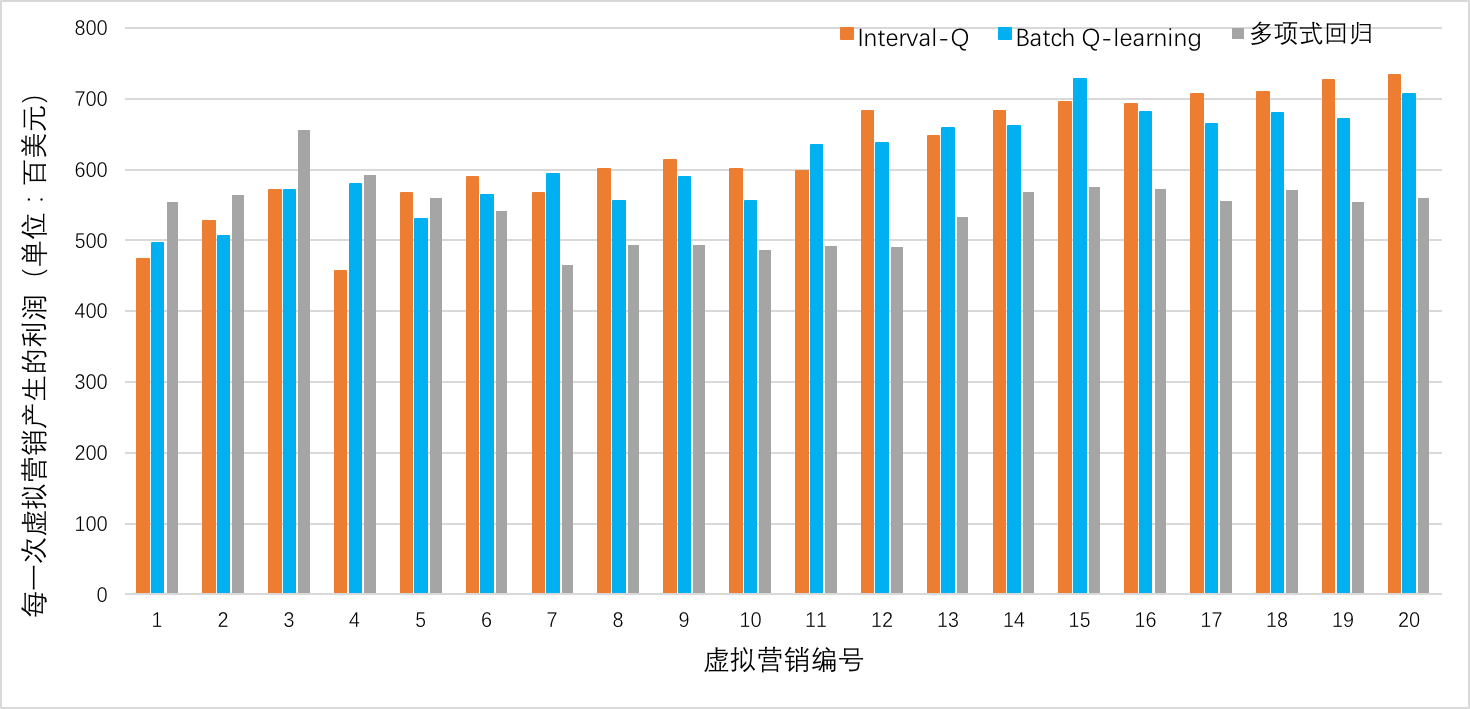
\includegraphics[width=1.0\textwidth]{e322}
\caption{每个虚拟营销中的总利润}
\label{fig:e322}
\end{figure}

首先,观察以上三个策略在20个虚拟营销过程中发送邮件的数量。从图\ref{fig:e321}中可以很明显地看出,Interval-Q和Batch Q-learning算法的营销策略在20个虚拟营销过程中所发送邮件的数量,远小于基于多项式回归算法的营销策略所发送邮件的数量。而Interval-Q算法的邮件数量(2070)比Batch Q-learning算法(2082)更少,从而说明Interval-Q算法有更好的成本控制能力。

% 但是,Interval-Q和Batch Q-learning算法在邮件发送数量上并没有多大区别。


接着,考察以上三个策略在20个虚拟营销过程中获得利润的变化情况。从图\ref{fig:e322}中可以看出,相比多项式回归方法,Interval-Q和Batch Q-learning算法在刚开始的几次虚拟营销中产生的利润比较低,但是在后续的营销中,其获得的利润在不断提升,这同样体现了强化学习方法在序贯决策问题中,因为考虑到了延迟影响并且以长期收益最大化作为学习目标,所以随着时间的推移,其产生的收益就会越来越高。而监督学习在学习中只考虑到了最大化即时收益,所以后续利润的增长就不是特别的明显。特别地,尽管Interval-Q和Batch Q-learning算法在20个虚拟营销中发送邮件的数量相似,但是Interval-Q算法所获得的总利润更高,特别是在最后的虚拟营销里,这主要归功于Interval-Q算法考虑到了时间间隔不固定的因素,因而可以更准确的进行值函数的逼近。

最后,结合图\ref{fig:e321}和图\ref{fig:e322}可以看出,尽管Interval-Q策略中第4次虚拟营销和Batch Q-learning策略中第5次虚拟营销,发送的邮件数量很少,但是仍然产生了很大的利润,而这个利润主要来源于之前营销活动的延迟反应。因为在该直邮营销的场景中,募捐者的延迟反馈会被记录到收到该反馈的那个日期里,而不是记录到发送该营销邮件的日期里,所以当在处理序列决策问题时,为了进行更有效的策略学习,应该考虑序列中的延迟影响,而这是监督学习方法很难办到的。另外,从图\ref{fig:e321}和图\ref{fig:e322}中可以看出,强化学习方法在制定营销策略的时候,是根据所采取的行为和收到的奖赏反馈来共同决定的。比如,在图\ref{fig:e321}中,Interval-Q算法在第3次发送邮件的数据相比第2次减少了,但是其产生的利润却增加了,所以在第4次制定营销策略的时候,Interval-Q算法就会有很大的概率选择继续减少邮件的数量,从图\ref{fig:e321}中也印证了这一点。

\begin{figure}[htbp]
\centering
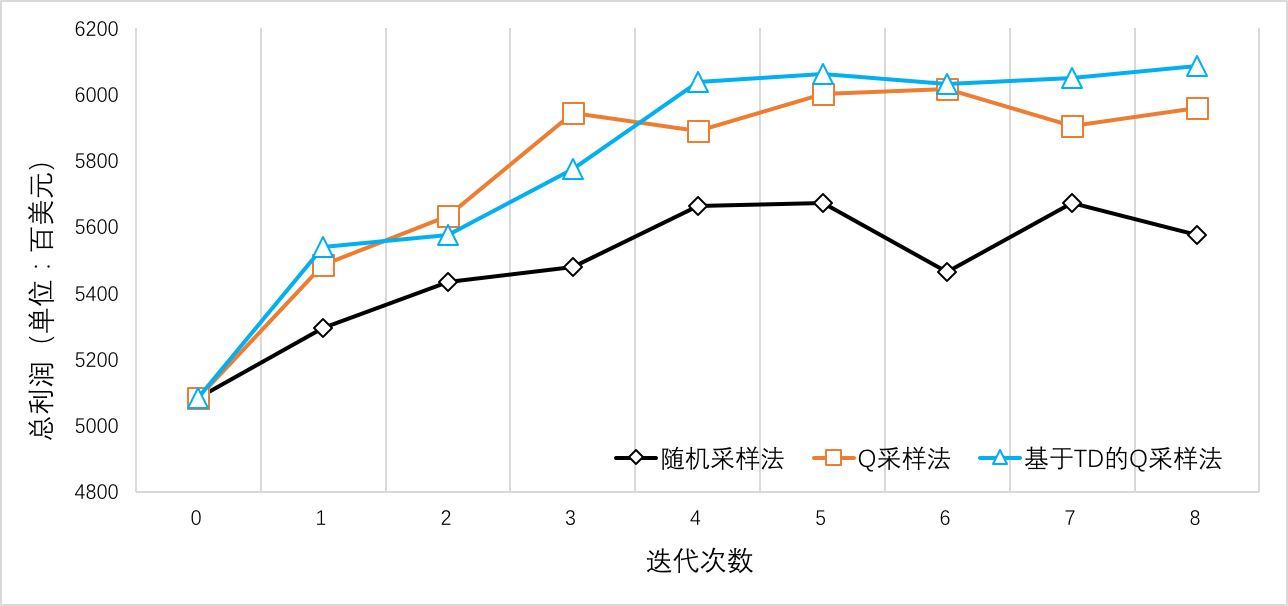
\includegraphics[width=1.0\textwidth]{e331}
\caption{不同采样方法下的利润}
\label{fig:e331}
\end{figure}

\begin{figure}[htbp]
\centering
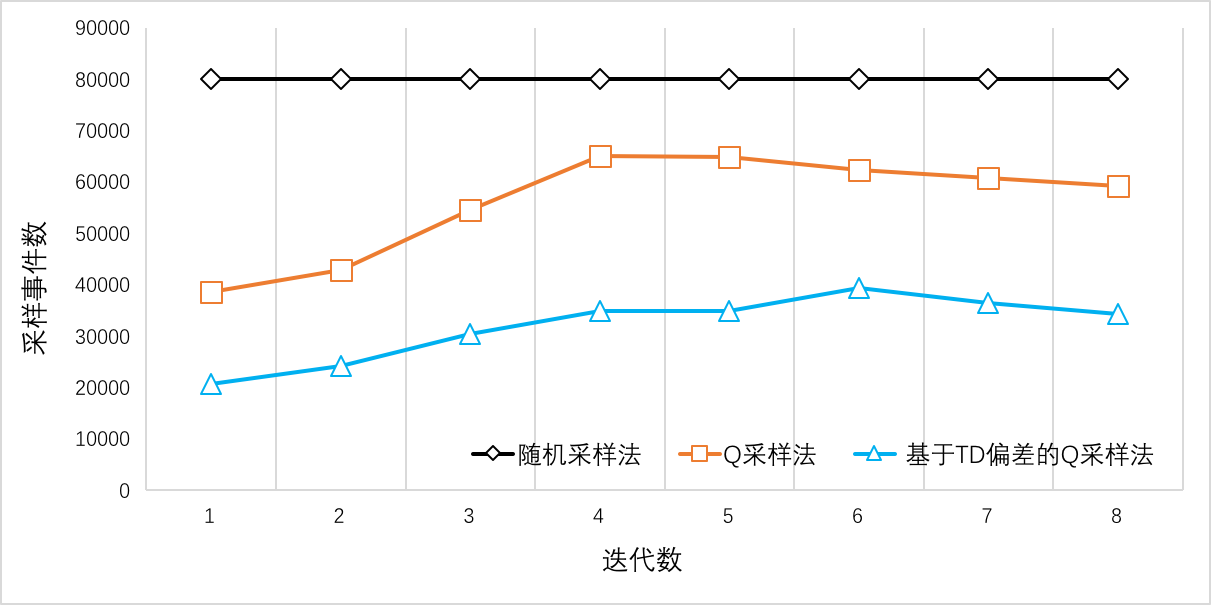
\includegraphics[width=1.0\textwidth]{e332}
\caption{不同采样方法下的采样数}
\label{fig:e332}
\end{figure}

\paragraph{采样方法比较}
最后,考察本文所提出的基于TD偏差的Q采样方法与Q采样法和随机采样法的效果对比,主要从采样数量和长期利润两个方面进行比较。在该实验中,选取一个规模大小为10000的情节集合,即160000个事件,在每轮迭代中随机抽取5000条情节(共80000个事件),然后再使用Q采样方法(算法:\ref{algo:SVR+Q_})和基于TD偏差的Q采样法(算法:\ref{algo:SVR+Q_2})进一步进行有条件采样。另外,在该实验中,基于TD偏差的Q采样法的阈值$\eta$设置为6.0。将每轮迭代所产生的利润平均值和所采样事件的数量记录下来,并绘制成图如\ref{fig:e331}和\ref{fig:e332}所示。

从图\ref{fig:e332}中可以看出,基于TD偏差的Q采样方法因为增加了TD偏差这一有效的约束条件,所以过滤掉了很多事件样本,其所采样的事件数量大约是Q采样方法的二分之一。不仅如此,从图\ref{fig:e331}可以看出,虽然基于TD偏差的Q采样方法采样数量下降了很多,但是其所获得的长期利润的能力却没有受到影响,甚至在最后几轮迭代的中,基于TD偏差的Q采样方法所产生的长期利润值超过了Q采样法。由此,可以得出,在面对数据规模比较大的现实应用中,基于TD偏差的Q采样法,在减少计算资源的情况也会学习到很好的策略。


\section{本章小结}
本章针对不定期直复营销场景中的营销时间间隔不固定,数据负载大导致学习速度慢的问题,基于传统的Q-learning算法进行改进。首先,给出直复营销在强化学习框架下的形式化描述以及基于Q-learning的算法模型,然后结合营销决策点间存在的时间间隔不固定问题,对Q-learning算法中值函数的更新方法进行改进,提出Interval-Q算法。接着,针对Interval-Q算法在处理大规模数据时的学习效率较低的问题,基于Q采样的方法,提出了基于TD偏差的Q采样方法。最后,介绍仿真环境的构建方法,并利用仿真环境从模型的长期收益、策略行为的变化以及采样方法的效果等三个方面对所提算法进行评估并对结果进行分析,评估结果验证了所提算法的有效性。

\cleardoublepage